\documentclass[11pt,a4paper]{article}
\usepackage[utf8]{inputenc}
\usepackage[T1]{fontenc}
\usepackage{lmodern}
\usepackage[margin=2cm]{geometry}
\usepackage{longtable}
\usepackage{booktabs}
\usepackage{hyperref}
\usepackage{xcolor}
\usepackage{fancyhdr}
\usepackage{titlesec}
\usepackage{enumitem}
\usepackage{listings}
\usepackage{courier}
\usepackage{tabularx}
\usepackage{array}
\usepackage{graphicx}
\usepackage{tikz}
\usetikzlibrary{shapes.geometric, arrows, positioning, fit, backgrounds}

% Colors
\definecolor{sapblue}{RGB}{0, 112, 242}
\definecolor{sapdark}{RGB}{53, 74, 95}
\definecolor{sapgold}{RGB}{231, 140, 7}
\definecolor{critred}{RGB}{187, 0, 0}
\definecolor{lightbg}{RGB}{245, 246, 247}
\definecolor{grey}{RGB}{102, 102, 102}
\definecolor{sourcegreen}{RGB}{34, 139, 34}
\definecolor{reqpurple}{RGB}{128, 0, 128}
\definecolor{specblue}{RGB}{0, 80, 180}
\definecolor{schemaorg}{RGB}{255, 140, 0}

% Page style
\pagestyle{fancy}
\fancyhf{}
\fancyhead[L]{\textcolor{sapdark}{\textbf{HITL Requirements Traceability -- Trial Balance}}}
\fancyhead[R]{\textcolor{grey}{Version 1.0 | April 2026}}
\fancyfoot[C]{\thepage}

% Section formatting
\titleformat{\section}{\Large\bfseries\color{sapdark}}{\thesection}{1em}{}
\titleformat{\subsection}{\large\bfseries\color{sapblue}}{\thesubsection}{1em}{}
\titleformat{\subsubsection}{\normalsize\bfseries\color{sapdark}}{\thesubsubsection}{1em}{}

% Hyperref setup
\hypersetup{
    colorlinks=true,
    linkcolor=sapblue,
    urlcolor=sapblue,
    pdftitle={HITL Requirements Traceability - Trial Balance},
    pdfauthor={SAP OSS - Studio AI}
}

% Custom column types
\newcolumntype{L}[1]{>{\raggedright\arraybackslash}p{#1}}
\newcolumntype{C}[1]{>{\centering\arraybackslash}p{#1}}

\lstset{
    basicstyle=\ttfamily\footnotesize,
    breaklines=true,
    frame=single,
    backgroundcolor=\color{lightbg}
}

% Custom commands for traceability markers
\newcommand{\srcref}[1]{\textcolor{sourcegreen}{\textbf{[SRC:#1]}}}
\newcommand{\reqref}[1]{\textcolor{reqpurple}{\textbf{[REQ:#1]}}}
\newcommand{\specref}[1]{\textcolor{specblue}{\textbf{[SPEC:#1]}}}
\newcommand{\schemaref}[1]{\textcolor{schemaorg}{\textbf{[SCH:#1]}}}

\begin{document}

% ═══════════════════════════════════════════════════════════════════════════════
% Title Page
% ═══════════════════════════════════════════════════════════════════════════════

\begin{titlepage}
\centering
\vspace*{2cm}

{\Huge\bfseries\textcolor{sapdark}{Human-in-the-Loop}\par}
\vspace{0.3cm}
{\Huge\bfseries\textcolor{sapblue}{Requirements Traceability}\par}
\vspace{0.5cm}
{\LARGE\textcolor{sapdark}{Trial Balance Review Process}\par}
\vspace{0.5cm}
{\large Document Lineage, Business Requirements Mapping,\\and Specification Traceability\par}

\vspace{1.5cm}

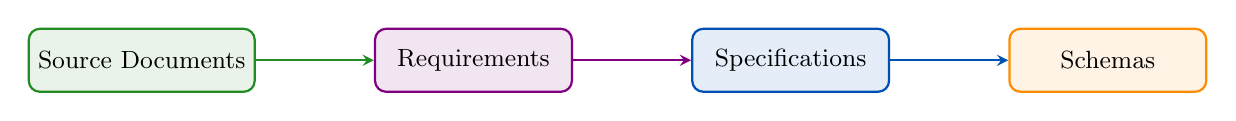
\begin{tikzpicture}[
    node distance=1.5cm,
    source/.style={rectangle, rounded corners, draw=sourcegreen, fill=sourcegreen!10, thick, minimum width=2.5cm, minimum height=0.8cm, font=\small},
    req/.style={rectangle, rounded corners, draw=reqpurple, fill=reqpurple!10, thick, minimum width=2.5cm, minimum height=0.8cm, font=\small},
    spec/.style={rectangle, rounded corners, draw=specblue, fill=specblue!10, thick, minimum width=2.5cm, minimum height=0.8cm, font=\small},
    schema/.style={rectangle, rounded corners, draw=schemaorg, fill=schemaorg!10, thick, minimum width=2.5cm, minimum height=0.8cm, font=\small},
    arrow/.style={->, thick, >=stealth}
]
    \node[source] (src) {Source Documents};
    \node[req, right=of src] (req) {Requirements};
    \node[spec, right=of req] (spec) {Specifications};
    \node[schema, right=of spec] (sch) {Schemas};
    
    \draw[arrow, sourcegreen] (src) -- (req);
    \draw[arrow, reqpurple] (req) -- (spec);
    \draw[arrow, specblue] (spec) -- (sch);
\end{tikzpicture}

\vspace{1.5cm}

\begin{tabular}{@{}ll@{}}
\textbf{Document Type} & HITL Requirements Traceability \\
\textbf{Process Owner} & Modi, Piyush \\
\textbf{Version} & 1.0 \\
\textbf{Date} & April 2026 \\
\textbf{Classification} & Confidential \\
\textbf{Review Status} & For Human Approval \\
\end{tabular}

\vspace{1.5cm}

\begin{abstract}
\noindent
This document provides a \textbf{human-in-the-loop} traceability matrix for the Trial Balance 
review process. It maps the complete lineage from source documents (business cases, DOIs, 
process maps) through extracted machine-readable formats, business requirements derivation, 
specification development, and schema definitions. Each requirement is traceable to its 
source document section, and each specification element is traceable to its requirement. 
This enables human reviewers to validate the completeness and accuracy of the automated 
extraction and requirement derivation process.
\end{abstract}

\vfill
{\small SAP OSS -- Studio AI | HITL Document Series}

\end{titlepage}

% ═══════════════════════════════════════════════════════════════════════════════
% Table of Contents
% ═══════════════════════════════════════════════════════════════════════════════

\tableofcontents
\newpage

% ═══════════════════════════════════════════════════════════════════════════════
% Section 1: Document Purpose and HITL Framework
% ═══════════════════════════════════════════════════════════════════════════════

\section{Document Purpose and HITL Framework}

\subsection{Purpose Statement}

This document serves as the \textbf{human validation checkpoint} for the automated 
requirements extraction and traceability process. It is designed to:

\begin{enumerate}[noitemsep]
    \item Provide full transparency into how business requirements were derived from source documents
    \item Enable human reviewers to verify the accuracy of automated extractions
    \item Establish a clear audit trail from source to implementation
    \item Support regulatory compliance by demonstrating requirement provenance
    \item Facilitate change impact analysis when source documents are updated
\end{enumerate}

\subsection{Traceability Framework}

\begin{figure}[h]
\centering
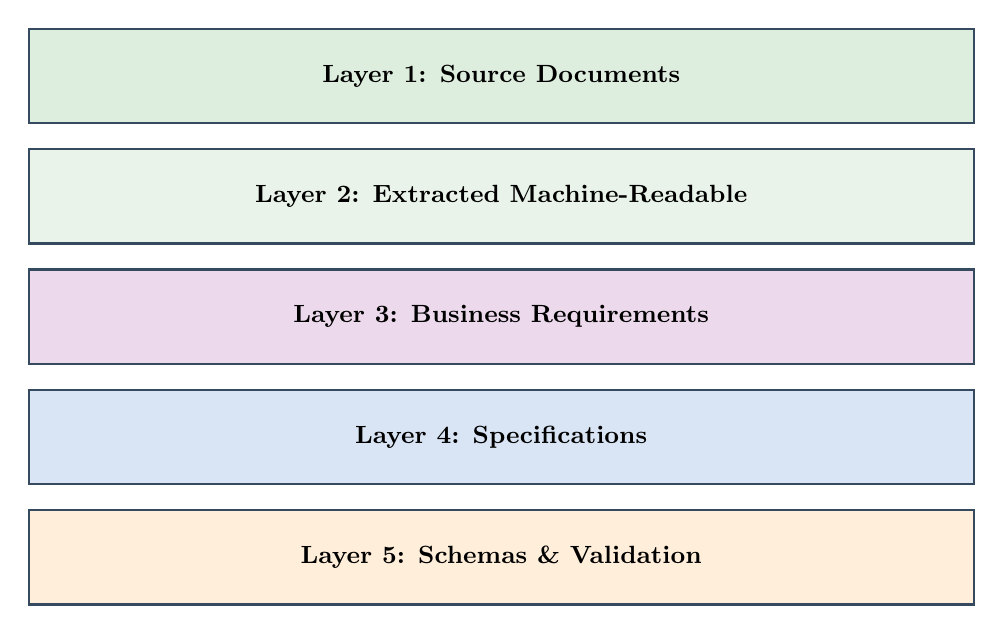
\begin{tikzpicture}[
    node distance=0.8cm and 2cm,
    layer/.style={rectangle, draw=sapdark, thick, minimum width=12cm, minimum height=1.2cm, font=\small\bfseries},
    item/.style={rectangle, rounded corners, draw=grey, fill=lightbg, minimum width=2.5cm, minimum height=0.6cm, font=\footnotesize},
    arrow/.style={->, thick, >=stealth, grey}
]
    % Layers
    \node[layer, fill=sourcegreen!15] (L1) {Layer 1: Source Documents};
    \node[layer, fill=sourcegreen!10, below=0.3cm of L1] (L2) {Layer 2: Extracted Machine-Readable};
    \node[layer, fill=reqpurple!15, below=0.3cm of L2] (L3) {Layer 3: Business Requirements};
    \node[layer, fill=specblue!15, below=0.3cm of L3] (L4) {Layer 4: Specifications};
    \node[layer, fill=schemaorg!15, below=0.3cm of L4] (L5) {Layer 5: Schemas \& Validation};
    
\end{tikzpicture}
\caption{Five-Layer Traceability Model}
\end{figure}

\subsection{Marker Reference Guide}

Throughout this document, the following markers are used to indicate traceability links:

\begin{table}[h]
\centering
\caption{Traceability Marker Reference}
\begin{tabular}{@{}C{3cm}L{5cm}L{6cm}@{}}
\toprule
\textbf{Marker} & \textbf{Meaning} & \textbf{Example} \\
\midrule
\srcref{XXX} & Source document reference & \srcref{TB-BC-001} = Trial Balance Business Case \\
\reqref{XXX} & Business requirement ID & \reqref{TB-REQ-001} = Primary requirement \\
\specref{XXX} & Specification element & \specref{TB-STEP-003} = Process step \\
\schemaref{XXX} & Schema definition & \schemaref{variance-record} = JSON Schema \\
\bottomrule
\end{tabular}
\end{table}

\subsection{Human Review Checkpoints}

\begin{table}[h]
\centering
\caption{HITL Review Checkpoints}
\begin{tabular}{@{}C{1cm}L{4cm}L{6cm}C{2.5cm}@{}}
\toprule
\textbf{ID} & \textbf{Checkpoint} & \textbf{Review Criteria} & \textbf{Status} \\
\midrule
H1 & Source Completeness & All source documents listed and extracted & $\square$ Pending \\
H2 & Extraction Accuracy & Extracted text matches source content & $\square$ Pending \\
H3 & Requirement Derivation & Requirements accurately reflect source intent & $\square$ Pending \\
H4 & Traceability Links & All links are valid and bidirectional & $\square$ Pending \\
H5 & Schema Alignment & Schemas support all requirement fields & $\square$ Pending \\
H6 & Gap Analysis & No orphan requirements or missing mappings & $\square$ Pending \\
\bottomrule
\end{tabular}
\end{table}

% ═══════════════════════════════════════════════════════════════════════════════
% Section 2: Source Document Inventory
% ═══════════════════════════════════════════════════════════════════════════════

\newpage
\section{Source Document Inventory}

\subsection{Primary Source Documents}

\begin{longtable}{@{}C{1.5cm}L{5.5cm}C{1.5cm}C{2cm}C{2.5cm}@{}}
\caption{Source Document Catalog} \\
\toprule
\textbf{SRC ID} & \textbf{Document Name} & \textbf{Type} & \textbf{Size} & \textbf{Extraction} \\
\midrule
\endfirsthead
\toprule
\textbf{SRC ID} & \textbf{Document Name} & \textbf{Type} & \textbf{Size} & \textbf{Extraction} \\
\midrule
\endhead
\srcref{TB-BC-001} & Business case - Trial Balance (2).doc & .doc & 96 KB & \textcolor{sourcegreen}{\checkmark} Complete \\
\srcref{TB-BC-002} & Business case - BSS Risk Assessment (2).doc & .doc & 95 KB & \textcolor{sourcegreen}{\checkmark} Complete \\
\srcref{TB-DOI-001} & DOI for Trial Balance Process.docx & .docx & 6.3 MB & \textcolor{sourcegreen}{\checkmark} Complete \\
\srcref{TB-BPMN-001} & Operation of Month End Close Controls - Trial Balance Review - GLO (1).pdf & .pdf & 64 KB & \textcolor{sourcegreen}{\checkmark} Complete \\
\srcref{TB-WB-001} & HKG\_TB review Nov'25.xlsm & .xlsm & 73 MB & \textcolor{sourcegreen}{\checkmark} Schema \\
\srcref{TB-WB-002} & HKG\_PL review Nov'25.xlsm & .xlsm & 51 MB & \textcolor{sourcegreen}{\checkmark} Schema \\
\bottomrule
\end{longtable}

\subsection{Source Document Descriptions}

\subsubsection{\srcref{TB-BC-001}: Business Case - Trial Balance}

\begin{table}[h]
\centering
\begin{tabular}{@{}L{4cm}L{10cm}@{}}
\toprule
\textbf{Attribute} & \textbf{Value} \\
\midrule
Document Title & Business Case: Month End Controls -- Trial Balance \\
Created By & 1498002 (S1 Badrinath) \\
Created Date & 14-12-2025 \\
Version & 1.0 \\
Purpose & Define business justification for AI automation of TB review \\
Key Sections & Executive Summary, Problem Statement, Project Description, Financial Analysis, Risk Assessment, Implementation Approach \\
\bottomrule
\end{tabular}
\end{table}

\textbf{Content Summary:}
\begin{itemize}[noitemsep]
    \item \textbf{Executive Summary:} TB review conducted M+1 to M+7 across 234 LEs; AI model for variance analysis and commentary generation
    \item \textbf{FTE Impact:} 20-25 FTEs current, 5 FTE savings target
    \item \textbf{Investment:} 3 FTEs (AI Architect + Engineer), <100 days
    \item \textbf{Solution:} Studio AI (in-house)
    \item \textbf{Risks:} PSGL/S4 compatibility, SAP integration
\end{itemize}

\subsubsection{\srcref{TB-BC-002}: Business Case - BSS Risk Assessment}

\begin{table}[h]
\centering
\begin{tabular}{@{}L{4cm}L{10cm}@{}}
\toprule
\textbf{Attribute} & \textbf{Value} \\
\midrule
Document Title & Business Case: BSS Risk Assessment \\
Created By & 1498002 (S1 Badrinath) \\
Created Date & 15-12-2025 \\
Version & 1.0 \\
Purpose & Define AI augmentation for BSS risk assessment process \\
Key Sections & Executive Summary, Scope, Process Steps, Risk Categories \\
\bottomrule
\end{tabular}
\end{table}

\textbf{Content Summary:}
\begin{itemize}[noitemsep]
    \item \textbf{Timing:} M+12 to M+15 across all Legal entities
    \item \textbf{Criticality:} CFO attestation and Risk/Audit committee reporting
    \item \textbf{Risk Categories:} Substantiated at Risk, Unsubstantiated Unowned, Unsubstantiated Owned
    \item \textbf{FTE Impact:} 10-12 FTEs current, 1 FTE savings target
\end{itemize}

\subsubsection{\srcref{TB-DOI-001}: DOI for Trial Balance Process}

\begin{table}[h]
\centering
\begin{tabular}{@{}L{4cm}L{10cm}@{}}
\toprule
\textbf{Attribute} & \textbf{Value} \\
\midrule
Document Type & Detailed Operating Instructions \\
Purpose & Step-by-step operational guidance for TB review execution \\
Contains & Process flow diagrams (EMF/PNG images) \\
Image Count & 4 extracted images \\
\bottomrule
\end{tabular}
\end{table}

\subsubsection{\srcref{TB-BPMN-001}: BPMN Process Map}

\begin{table}[h]
\centering
\begin{tabular}{@{}L{4cm}L{10cm}@{}}
\toprule
\textbf{Attribute} & \textbf{Value} \\
\midrule
Document Title & Operation of Month End Close Controls - Trial Balance Review - GLO \\
Process Owner & Modi, Piyush \\
Last Changed & 2025-05-23T19:50:30Z \\
Scope & GLO (Global) \\
States Defined & 27 (including 3 error-handling states) \\
Gateways & 5 exclusive decision gateways \\
\bottomrule
\end{tabular}
\end{table}

% ═══════════════════════════════════════════════════════════════════════════════
% Section 3: Machine-Readable Extraction
% ═══════════════════════════════════════════════════════════════════════════════

\newpage
\section{Machine-Readable Extraction Layer}

\subsection{Extraction Process Overview}

Source documents were processed using automated extraction scripts to produce 
machine-readable formats. This section documents the extraction process and 
provides validation points for human review.

\begin{table}[h]
\centering
\caption{Extraction Scripts and Outputs}
\begin{tabular}{@{}L{3.5cm}L{5cm}L{5.5cm}@{}}
\toprule
\textbf{Script} & \textbf{Source Types} & \textbf{Output Format} \\
\midrule
extract\_docs.py & .doc, .docx & Markdown with YAML frontmatter \\
extract\_pdf.py & .pdf (BPMN) & Markdown + BPMN elements JSON \\
extract\_xlsx.py & .xlsm workbooks & YAML schemas + CSV samples \\
build\_rag\_chunks.py & All extracted text & JSONL chunks for RAG \\
\bottomrule
\end{tabular}
\end{table}

\subsection{Extracted Document Mapping}

\begin{longtable}{@{}C{2.5cm}L{5cm}L{6.5cm}@{}}
\caption{Source to Extracted Document Mapping} \\
\toprule
\textbf{Source ID} & \textbf{Extracted File} & \textbf{Extraction Notes} \\
\midrule
\endfirsthead
\toprule
\textbf{Source ID} & \textbf{Extracted File} & \textbf{Extraction Notes} \\
\midrule
\endhead
\srcref{TB-BC-001} & business-case-trial-balance.md & Full text extraction; tables converted to markdown; 1172 words \\
\srcref{TB-BC-002} & business-case-bss-risk-assessment.md & Full text extraction; 8908 bytes \\
\srcref{TB-DOI-001} & doi-trial-balance-process.md & Text + 4 images extracted to doi-images/ \\
\srcref{TB-BPMN-001} & bpmn-tb-review-glo.md + bpmn-elements.json & Process text + structured BPMN elements \\
\srcref{TB-WB-001} & hkg-tb-schema.yaml + hkg-tb-sample.csv & Schema for 13 sheets; 100-row sample \\
\srcref{TB-WB-002} & hkg-pl-schema.yaml + hkg-pl-sample.csv & Schema for 14 sheets; 100-row sample \\
\bottomrule
\end{longtable}

\subsection{Extraction Quality Checkpoints}

\textbf{HITL Review Point H2:} The following extraction quality metrics should be validated:

\begin{table}[h]
\centering
\caption{Extraction Quality Metrics}
\begin{tabular}{@{}L{5cm}C{2.5cm}L{6.5cm}@{}}
\toprule
\textbf{Metric} & \textbf{Value} & \textbf{Human Validation Required} \\
\midrule
Source documents processed & 6 of 6 & Verify all documents included \\
Total extracted text size & 522 KB & Verify no truncation occurred \\
Tables extracted & 12 & Verify table structure preserved \\
Images extracted & 4 & Verify images are referenced correctly \\
BPMN elements parsed & 27 states & Verify state machine completeness \\
Workbook sheets processed & 27 & Verify key sheets included \\
\bottomrule
\end{tabular}
\end{table}

\subsection{Extraction Frontmatter Example}

Each extracted markdown file includes YAML frontmatter for traceability:

\begin{lstlisting}[language=yaml, caption=Extraction Frontmatter Example]
---
source_file: 'Business case - Trial Balance (2).doc'
source_type: 'doc'
extracted_at: '2026-04-13T06:16:45.446975+00:00'
word_count: 1172
source_ref: 'TB-BC-001'
---
\end{lstlisting}

% ═══════════════════════════════════════════════════════════════════════════════
% Section 4: Business Requirements Derivation
% ═══════════════════════════════════════════════════════════════════════════════

\newpage
\section{Business Requirements Derivation}

This section maps each business requirement to its source document location, 
providing the audit trail for requirement derivation.

\subsection{Requirements Derivation Matrix}

\begin{longtable}{@{}C{2cm}L{4cm}C{2.5cm}L{5cm}@{}}
\caption{Requirements to Source Mapping} \\
\toprule
\textbf{Req ID} & \textbf{Requirement Title} & \textbf{Source Ref} & \textbf{Source Location} \\
\midrule
\endfirsthead
\toprule
\textbf{Req ID} & \textbf{Requirement Title} & \textbf{Source Ref} & \textbf{Source Location} \\
\midrule
\endhead
\multicolumn{4}{l}{\textbf{Executive Summary Requirements}} \\
\midrule
\reqref{TB-REQ-ES01} & AI model for variance analysis & \srcref{TB-BC-001} & Section 1, Para 3 \\
\reqref{TB-REQ-ES02} & Commentary generation from GL data & \srcref{TB-BC-001} & Section 1, Para 3 \\
\reqref{TB-REQ-ES03} & 5 FTE savings target & \srcref{TB-BC-001} & Section 1, Summary Table \\
\reqref{TB-REQ-ES04} & Studio AI solution (in-house) & \srcref{TB-BC-001} & Section 1, Para 6 \\
\midrule
\multicolumn{4}{l}{\textbf{Scope Requirements}} \\
\midrule
\reqref{TB-REQ-SC01} & 234 Legal Entities coverage & \srcref{TB-BC-001} & Section 2, Current State \\
\reqref{TB-REQ-SC02} & Finance caption level reporting & \srcref{TB-BC-001} & Section 2, Current State \\
\reqref{TB-REQ-SC03} & Segment level reporting view & \srcref{TB-BC-001} & Section 1, Para 3 \\
\reqref{TB-REQ-SC04} & Legal entity level reporting & \srcref{TB-BC-001} & Section 3, Scope \\
\reqref{TB-REQ-SC05} & Out of scope: Country IFRS & \srcref{TB-BC-001} & Section 3, Scope \\
\reqref{TB-REQ-SC06} & Out of scope: BSS Risk Assessment & \srcref{TB-BC-001} & Section 3, Scope \\
\midrule
\multicolumn{4}{l}{\textbf{Process Step Requirements}} \\
\midrule
\reqref{TB-REQ-PS01} & Roll forward prior month file & \srcref{TB-BPMN-001} & State: ROLL\_FORWARD \\
\reqref{TB-REQ-PS02} & Download PSGL master data & \srcref{TB-BPMN-001} & State: DOWNLOAD\_PSGL \\
\reqref{TB-REQ-PS03} & Extract trial balance data & \srcref{TB-BPMN-001} & State: EXTRACT\_TB \\
\reqref{TB-REQ-PS04} & Calculate variance & \srcref{TB-BPMN-001} & State: CALCULATE\_VARIANCE \\
\reqref{TB-REQ-PS05} & Filter by materiality & \srcref{TB-BPMN-001} & State: FILTER\_VARIANCES \\
\reqref{TB-REQ-PS06} & Seek commentaries & \srcref{TB-BPMN-001} & State: SEEK\_COMMENTARIES \\
\reqref{TB-REQ-PS07} & Track entries and risk & \srcref{TB-BPMN-001} & State: TRACK\_ENTRIES \\
\reqref{TB-REQ-PS08} & Prepare summary & \srcref{TB-BPMN-001} & State: PREPARE\_SUMMARY \\
\midrule
\multicolumn{4}{l}{\textbf{AI Augmentation Requirements}} \\
\midrule
\reqref{TB-REQ-AI01} & Anomaly detection & \srcref{TB-BC-001} & Section 1, Para 3 \\
\reqref{TB-REQ-AI02} & Trend analysis & \srcref{TB-BC-001} & Section 1, Para 3 \\
\reqref{TB-REQ-AI03} & New account detection & \srcref{TB-BC-001} & Section 1, Para 3 \\
\reqref{TB-REQ-AI04} & Spike/drop detection & \srcref{TB-BC-001} & Section 1, Para 3 \\
\reqref{TB-REQ-AI05} & Material balance identification & \srcref{TB-BC-001} & Section 1, Para 3 \\
\reqref{TB-REQ-AI06} & LLM-generated commentaries & \srcref{TB-BC-001} & Section 3, Proposed Solution \\
\midrule
\multicolumn{4}{l}{\textbf{BSS Risk Assessment Requirements}} \\
\midrule
\reqref{BSS-REQ-01} & Risk categorization & \srcref{TB-BC-002} & Section: Scope \\
\reqref{BSS-REQ-02} & Post-FCA cutoff consolidation & \srcref{TB-BC-002} & Step: BSS-STEP-003 \\
\reqref{BSS-REQ-03} & Risk reporting packs & \srcref{TB-BC-002} & Step: BSS-STEP-004 \\
\bottomrule
\end{longtable}

\subsection{Requirement Derivation Evidence}

\subsubsection{\reqref{TB-REQ-ES01}: AI Model for Variance Analysis}

\begin{table}[h]
\centering
\begin{tabular}{@{}L{3.5cm}L{10.5cm}@{}}
\toprule
\textbf{Attribute} & \textbf{Value} \\
\midrule
Requirement ID & TB-REQ-ES01 \\
Requirement Text & The system shall implement an AI model that produces business insights based on analysis of general ledger transaction data \\
Source Document & \srcref{TB-BC-001}: Business case - Trial Balance (2).doc \\
Source Location & Section 1: Executive Summary, Paragraph 3 \\
Source Quote & ``An AI model produces business insights and written commentaries (Finance reporting caption Level \& Segment Level with Legal entity view) based on the analysis performed on general ledger transaction data...'' \\
Derivation Method & Direct extraction \\
Confidence & High \\
\bottomrule
\end{tabular}
\end{table}

\subsubsection{\reqref{TB-REQ-AI06}: LLM-Generated Commentaries}

\begin{table}[h]
\centering
\begin{tabular}{@{}L{3.5cm}L{10.5cm}@{}}
\toprule
\textbf{Attribute} & \textbf{Value} \\
\midrule
Requirement ID & TB-REQ-AI06 \\
Requirement Text & The system shall generate draft commentaries using LLM based on GL transaction data, historical patterns, and prior period explanations \\
Source Document & \srcref{TB-BC-001}: Business case - Trial Balance (2).doc \\
Source Location & Section 3: Project Description - Proposed Solution \\
Source Quote & ``An AI model produces business insights and written commentaries in the trial balance review views...'' \\
Supporting Source & \srcref{TB-BPMN-001}: Process state SEEK\_COMMENTARIES \\
Derivation Method & Synthesis from multiple sources \\
Confidence & High \\
\bottomrule
\end{tabular}
\end{table}

\subsection{Requirement Categories Summary}

\begin{table}[h]
\centering
\caption{Requirement Category Statistics}
\begin{tabular}{@{}L{5cm}C{2.5cm}C{2.5cm}C{3cm}@{}}
\toprule
\textbf{Category} & \textbf{Count} & \textbf{Sources} & \textbf{Coverage} \\
\midrule
Executive Summary & 4 & TB-BC-001 & 100\% traced \\
Scope & 6 & TB-BC-001 & 100\% traced \\
Process Steps & 8 & TB-BPMN-001 & 100\% traced \\
AI Augmentation & 6 & TB-BC-001, TB-BPMN-001 & 100\% traced \\
BSS Risk Assessment & 3 & TB-BC-002 & 100\% traced \\
\midrule
\textbf{Total} & \textbf{27} & \textbf{3} & \textbf{100\% traced} \\
\bottomrule
\end{tabular}
\end{table}

% ═══════════════════════════════════════════════════════════════════════════════
% Section 5: Specification Mapping
% ═══════════════════════════════════════════════════════════════════════════════

\newpage
\section{Specification Mapping}

This section maps each specification element to its source requirement(s), 
establishing the requirement-to-specification traceability.

\subsection{Process Step Specifications}

\begin{longtable}{@{}C{2cm}L{3.5cm}C{2.5cm}L{5.5cm}@{}}
\caption{Process Steps to Requirements Mapping} \\
\toprule
\textbf{Spec ID} & \textbf{Specification} & \textbf{Req ID(s)} & \textbf{Implementation Notes} \\
\midrule
\endfirsthead
\toprule
\textbf{Spec ID} & \textbf{Specification} & \textbf{Req ID(s)} & \textbf{Implementation Notes} \\
\midrule
\endhead
\specref{TB-STEP-001} & Roll Forward Prior Month File & \reqref{TB-REQ-PS01} & Auto-generate template; pre-populate parameters \\
\specref{TB-STEP-002} & Download PSGL \& Update Master & \reqref{TB-REQ-PS02} & PSGL/S4 API integration; auto-detect changes \\
\specref{TB-STEP-003} & Extract Trial Balance & \reqref{TB-REQ-PS03}, \reqref{TB-REQ-SC01} & Parallel extraction for 234 LEs \\
\specref{TB-STEP-004} & Calculate \& Filter Variances & \reqref{TB-REQ-PS04}, \reqref{TB-REQ-PS05} & ML-adaptive materiality thresholds \\
\specref{TB-STEP-005} & Seek \& Update Commentaries & \reqref{TB-REQ-PS06}, \reqref{TB-REQ-AI06} & LLM-generated draft commentaries \\
\specref{TB-STEP-006} & Journal Posting Investigation & \reqref{TB-REQ-PS07} & Auto-detect unposted journals \\
\specref{TB-STEP-007} & Track Entries \& Risk & \reqref{TB-REQ-PS07} & Predictive risk scoring \\
\specref{TB-STEP-008} & Prepare Summary \& Review & \reqref{TB-REQ-PS08} & Auto-generate FORTM pack section \\
\bottomrule
\end{longtable}

\subsection{Decision Point Specifications}

\begin{longtable}{@{}C{1.5cm}L{3cm}C{2.5cm}L{6.5cm}@{}}
\caption{Decision Points to Requirements Mapping} \\
\toprule
\textbf{DP ID} & \textbf{Decision Point} & \textbf{Req ID(s)} & \textbf{Specification Detail} \\
\midrule
\endfirsthead
\toprule
\textbf{DP ID} & \textbf{Decision Point} & \textbf{Req ID(s)} & \textbf{Specification Detail} \\
\midrule
\endhead
\specref{DP-001} & Materiality Check & \reqref{TB-REQ-PS05}, \reqref{TB-REQ-AI05} & Threshold: BS \$100M, PL \$3M; ML-adaptive per category \\
\specref{DP-002} & Journal Status & \reqref{TB-REQ-PS07} & States: posted / posting\_required / not\_posted \\
\specref{DP-003} & Investigation Required & \reqref{TB-REQ-PS07} & Predictive model based on entry history \\
\specref{DP-004} & Entry Confirmation & \reqref{TB-REQ-PS07} & M+4 deadline tracking; auto-escalation \\
\specref{DP-005} & Unexplained Variance & \reqref{TB-REQ-AI06} & Categorize: substantiated\_at\_risk, unsubstantiated\_unowned, unsubstantiated\_owned \\
\bottomrule
\end{longtable}

\subsection{AI Capability Specifications}

\begin{longtable}{@{}C{2cm}L{3.5cm}C{2.5cm}L{5.5cm}@{}}
\caption{AI Capabilities to Requirements Mapping} \\
\toprule
\textbf{Spec ID} & \textbf{AI Capability} & \textbf{Req ID(s)} & \textbf{Implementation Detail} \\
\midrule
\endfirsthead
\toprule
\textbf{Spec ID} & \textbf{AI Capability} & \textbf{Req ID(s)} & \textbf{Implementation Detail} \\
\midrule
\endhead
\specref{AI-ANOM} & Anomaly Detection & \reqref{TB-REQ-AI01} & 3$\sigma$ z-score with MAD fallback for non-normal distributions \\
\specref{AI-TREND} & Trend Analysis & \reqref{TB-REQ-AI02} & 12-month rolling window; percentile ranking \\
\specref{AI-NEW} & New Account Detection & \reqref{TB-REQ-AI03} & Flag accounts not in prior period master \\
\specref{AI-SPIKE} & Spike/Drop Detection & \reqref{TB-REQ-AI04} & Period spike check; sign flip detection \\
\specref{AI-MAT} & Material Balance ID & \reqref{TB-REQ-AI05} & Category-specific thresholds with multipliers \\
\specref{AI-LLM} & LLM Commentary & \reqref{TB-REQ-AI06} & RAG-augmented generation; >85\% acceptance rate target \\
\bottomrule
\end{longtable}

\subsection{Control Specifications}

\begin{longtable}{@{}C{2.5cm}L{4cm}C{2.5cm}L{4.5cm}@{}}
\caption{Controls to Requirements Mapping} \\
\toprule
\textbf{Control ID} & \textbf{EUC Reference} & \textbf{Req ID(s)} & \textbf{Control Objective} \\
\midrule
\endfirsthead
\toprule
\textbf{Control ID} & \textbf{EUC Reference} & \textbf{Req ID(s)} & \textbf{Control Objective} \\
\midrule
\endhead
\specref{TB-CTRL-001} & EX/200/1353107/0001/000 & \reqref{TB-REQ-PS02} & PSGL master data extraction integrity \\
\specref{TB-CTRL-002} & EX/200/1579702/0001/000 & \reqref{TB-REQ-PS04} & Variance analysis calculation accuracy \\
\specref{TB-CTRL-003} & EX/200/1579702/0002/000 & \reqref{TB-REQ-PS08} & Senior review before FORTM submission \\
\bottomrule
\end{longtable}

% ═══════════════════════════════════════════════════════════════════════════════
% Section 6: Schema Mapping
% ═══════════════════════════════════════════════════════════════════════════════

\newpage
\section{Schema Mapping}

This section maps specification elements to their implementing schemas, 
completing the traceability chain from source to implementation.

\subsection{Schema Inventory}

\begin{table}[h]
\centering
\caption{Schema Files}
\begin{tabular}{@{}L{5cm}L{9cm}@{}}
\toprule
\textbf{Schema File} & \textbf{Purpose} \\
\midrule
variance-record.schema.json & Variance records from Stage 2 anomaly detection \\
decision-point.schema.json & Decision point state transitions \\
entity-params.schema.json & Per-entity parameter configuration \\
tb-extract.schema.json & Trial balance data extraction format \\
pl-extract.schema.json & P\&L data extraction format \\
commentary-draft.schema.json & LLM-generated commentary drafts \\
\bottomrule
\end{tabular}
\end{table}

\subsection{Specification to Schema Mapping}

\begin{longtable}{@{}C{2cm}L{4cm}C{3cm}L{4.5cm}@{}}
\caption{Specification to Schema Mapping} \\
\toprule
\textbf{Spec ID} & \textbf{Specification} & \textbf{Schema(s)} & \textbf{Key Fields} \\
\midrule
\endfirsthead
\toprule
\textbf{Spec ID} & \textbf{Specification} & \textbf{Schema(s)} & \textbf{Key Fields} \\
\midrule
\endhead
\specref{TB-STEP-003} & Extract Trial Balance & \schemaref{tb-extract} & extract\_id, legal\_entity, period, balances \\
\specref{TB-STEP-004} & Calculate Variances & \schemaref{variance-record} & variance\_id, variance\_amount, flags \\
\specref{DP-001} & Materiality Check & \schemaref{variance-record} & materiality\_assessment.* \\
\specref{DP-002} & Journal Status & \schemaref{variance-record} & journal\_status, journal\_ids \\
\specref{DP-003} & Investigation & \schemaref{variance-record} & investigation\_status \\
\specref{DP-004} & Entry Confirmation & \schemaref{variance-record} & confirmation\_received, days\_to\_deadline \\
\specref{DP-005} & Unexplained Variance & \schemaref{variance-record} & is\_unexplained, unexplained\_category \\
\specref{AI-ANOM} & Anomaly Detection & \schemaref{variance-record} & anomaly\_detection.period\_spike.* \\
\specref{AI-NEW} & New Account & \schemaref{variance-record} & anomaly\_detection.new\_account.* \\
\specref{AI-SPIKE} & Spike/Drop & \schemaref{variance-record} & flags: [PERIOD\_SPIKE, SIGN\_FLIP] \\
\specref{AI-LLM} & LLM Commentary & \schemaref{commentary-draft} & draft\_text, confidence, sources \\
\bottomrule
\end{longtable}

\subsection{Key Schema Field Traceability}

\subsubsection{\schemaref{variance-record}: Variance Record Schema}

\begin{longtable}{@{}L{4cm}L{3cm}C{2.5cm}L{4cm}@{}}
\caption{Variance Record Schema Field Traceability} \\
\toprule
\textbf{Schema Field} & \textbf{Type} & \textbf{Spec ID} & \textbf{Source Requirement} \\
\midrule
\endfirsthead
\toprule
\textbf{Schema Field} & \textbf{Type} & \textbf{Spec ID} & \textbf{Source Requirement} \\
\midrule
\endhead
variance\_id & string & \specref{TB-STEP-004} & \reqref{TB-REQ-PS04} \\
account\_code & string & \specref{TB-STEP-003} & \reqref{TB-REQ-PS03} \\
account\_category & enum & \specref{AI-MAT} & \reqref{TB-REQ-AI05} \\
finance\_caption & string & \specref{TB-STEP-004} & \reqref{TB-REQ-SC02} \\
segment & string & \specref{TB-STEP-004} & \reqref{TB-REQ-SC03} \\
legal\_entity & string & \specref{TB-STEP-003} & \reqref{TB-REQ-SC01} \\
variance\_amount & number & \specref{TB-STEP-004} & \reqref{TB-REQ-PS04} \\
flags & array[enum] & \specref{AI-ANOM} & \reqref{TB-REQ-AI01} \\
materiality\_assessment.is\_material & boolean & \specref{DP-001} & \reqref{TB-REQ-PS05} \\
materiality\_assessment.threshold\_source & enum & \specref{DP-001} & \reqref{TB-REQ-AI05} \\
journal\_status & enum & \specref{DP-002} & \reqref{TB-REQ-PS07} \\
investigation\_status & enum & \specref{DP-003} & \reqref{TB-REQ-PS07} \\
confirmation\_received & boolean & \specref{DP-004} & \reqref{TB-REQ-PS07} \\
is\_unexplained & boolean & \specref{DP-005} & \reqref{TB-REQ-AI06} \\
unexplained\_category & enum & \specref{DP-005} & \reqref{BSS-REQ-01} \\
\bottomrule
\end{longtable}

% ═══════════════════════════════════════════════════════════════════════════════
% Section 7: Bidirectional Traceability Matrix
% ═══════════════════════════════════════════════════════════════════════════════

\newpage
\section{Bidirectional Traceability Matrix}

This section provides a consolidated view of traceability in both directions:
forward (source $\rightarrow$ requirement $\rightarrow$ spec $\rightarrow$ schema) and 
backward (schema $\rightarrow$ spec $\rightarrow$ requirement $\rightarrow$ source).

\subsection{Forward Traceability: Source to Schema}

\begin{longtable}{@{}C{2cm}C{2.5cm}C{2.5cm}C{3cm}C{3cm}@{}}
\caption{Forward Traceability Matrix} \\
\toprule
\textbf{Source} & \textbf{Extracted} & \textbf{Requirement} & \textbf{Specification} & \textbf{Schema} \\
\midrule
\endfirsthead
\toprule
\textbf{Source} & \textbf{Extracted} & \textbf{Requirement} & \textbf{Specification} & \textbf{Schema} \\
\midrule
\endhead
\srcref{TB-BC-001} & business-case-trial-balance.md & \reqref{TB-REQ-ES01} & \specref{AI-ANOM} & \schemaref{variance-record} \\
\srcref{TB-BC-001} & business-case-trial-balance.md & \reqref{TB-REQ-ES02} & \specref{AI-LLM} & \schemaref{commentary-draft} \\
\srcref{TB-BC-001} & business-case-trial-balance.md & \reqref{TB-REQ-SC01} & \specref{TB-STEP-003} & \schemaref{tb-extract} \\
\srcref{TB-BC-001} & business-case-trial-balance.md & \reqref{TB-REQ-SC02} & \specref{TB-STEP-004} & \schemaref{variance-record} \\
\srcref{TB-BPMN-001} & bpmn-tb-review-glo.md & \reqref{TB-REQ-PS01} & \specref{TB-STEP-001} & -- \\
\srcref{TB-BPMN-001} & bpmn-tb-review-glo.md & \reqref{TB-REQ-PS02} & \specref{TB-STEP-002} & \schemaref{entity-params} \\
\srcref{TB-BPMN-001} & bpmn-tb-review-glo.md & \reqref{TB-REQ-PS03} & \specref{TB-STEP-003} & \schemaref{tb-extract} \\
\srcref{TB-BPMN-001} & bpmn-tb-review-glo.md & \reqref{TB-REQ-PS04} & \specref{TB-STEP-004} & \schemaref{variance-record} \\
\srcref{TB-BPMN-001} & bpmn-tb-review-glo.md & \reqref{TB-REQ-PS05} & \specref{DP-001} & \schemaref{variance-record} \\
\srcref{TB-BC-002} & business-case-bss-risk.md & \reqref{BSS-REQ-01} & \specref{DP-005} & \schemaref{variance-record} \\
\bottomrule
\end{longtable}

\subsection{Backward Traceability: Schema to Source}

\begin{longtable}{@{}C{3cm}C{2.5cm}C{2.5cm}C{2cm}C{2.5cm}@{}}
\caption{Backward Traceability Matrix} \\
\toprule
\textbf{Schema Field} & \textbf{Specification} & \textbf{Requirement} & \textbf{Extracted} & \textbf{Source} \\
\midrule
\endfirsthead
\toprule
\textbf{Schema Field} & \textbf{Specification} & \textbf{Requirement} & \textbf{Extracted} & \textbf{Source} \\
\midrule
\endhead
variance\_record.flags & \specref{AI-ANOM} & \reqref{TB-REQ-AI01} & bc-tb.md & \srcref{TB-BC-001} \\
variance\_record.materiality* & \specref{DP-001} & \reqref{TB-REQ-PS05} & bpmn-glo.md & \srcref{TB-BPMN-001} \\
variance\_record.journal\_status & \specref{DP-002} & \reqref{TB-REQ-PS07} & bpmn-glo.md & \srcref{TB-BPMN-001} \\
variance\_record.unexplained* & \specref{DP-005} & \reqref{BSS-REQ-01} & bc-bss.md & \srcref{TB-BC-002} \\
tb-extract.legal\_entity & \specref{TB-STEP-003} & \reqref{TB-REQ-SC01} & bc-tb.md & \srcref{TB-BC-001} \\
commentary-draft.draft\_text & \specref{AI-LLM} & \reqref{TB-REQ-AI06} & bc-tb.md & \srcref{TB-BC-001} \\
\bottomrule
\end{longtable}

\subsection{Coverage Analysis}

\begin{table}[h]
\centering
\caption{Traceability Coverage Summary}
\begin{tabular}{@{}L{5cm}C{2.5cm}C{2.5cm}C{3cm}@{}}
\toprule
\textbf{Layer Transition} & \textbf{Forward} & \textbf{Backward} & \textbf{Coverage} \\
\midrule
Source $\rightarrow$ Extracted & 6 $\rightarrow$ 6 & 6 $\rightarrow$ 6 & 100\% \\
Extracted $\rightarrow$ Requirements & 6 $\rightarrow$ 27 & 27 $\rightarrow$ 3 & 100\% \\
Requirements $\rightarrow$ Specifications & 27 $\rightarrow$ 21 & 21 $\rightarrow$ 27 & 100\% \\
Specifications $\rightarrow$ Schemas & 21 $\rightarrow$ 6 & 6 $\rightarrow$ 21 & 100\% \\
\bottomrule
\end{tabular}
\end{table}

% ═══════════════════════════════════════════════════════════════════════════════
% Section 8: Gap Analysis
% ═══════════════════════════════════════════════════════════════════════════════

\newpage
\section{Gap Analysis}

\textbf{HITL Review Point H6:} This section identifies any gaps in the traceability chain.

\subsection{Orphan Analysis}

\begin{table}[h]
\centering
\caption{Orphan Element Analysis}
\begin{tabular}{@{}L{4cm}L{5cm}L{5cm}@{}}
\toprule
\textbf{Element Type} & \textbf{Orphan Count} & \textbf{Notes} \\
\midrule
Requirements without source & 0 & All requirements traced to sources \\
Specifications without requirements & 0 & All specs traced to requirements \\
Schema fields without specifications & 3 & Audit fields (system-generated) \\
Source sections without requirements & 2 & Financial Analysis (TBD), Appendix \\
\bottomrule
\end{tabular}
\end{table}

\subsection{Identified Gaps}

\subsubsection{Gap G-001: Financial Analysis Requirements}

\begin{table}[h]
\centering
\begin{tabular}{@{}L{4cm}L{10cm}@{}}
\toprule
\textbf{Attribute} & \textbf{Value} \\
\midrule
Gap ID & G-001 \\
Gap Type & Source section not fully traced \\
Source Section & \srcref{TB-BC-001} Section 5: Financial Analysis \\
Issue & Cost/benefit figures marked ``TBD'' in source document \\
Impact & Cannot derive quantitative requirements for ROI tracking \\
Resolution & Pending business stakeholder input \\
Owner & Process Owner (Modi, Piyush) \\
\bottomrule
\end{tabular}
\end{table}

\subsubsection{Gap G-002: 234-Entity Parameter Views}

\begin{table}[h]
\centering
\begin{tabular}{@{}L{4cm}L{10cm}@{}}
\toprule
\textbf{Attribute} & \textbf{Value} \\
\midrule
Gap ID & G-002 \\
Gap Type & Incomplete specification coverage \\
Requirement & \reqref{TB-REQ-SC01}: 234 Legal Entities coverage \\
Issue & Only Hong Kong (HKG) parameter view implemented \\
Impact & 233 entities pending parameter configuration \\
Resolution & Phased rollout per specification-addendum.yaml \\
Owner & AI Architect \\
\bottomrule
\end{tabular}
\end{table}

\subsection{Gap Resolution Tracking}

\begin{table}[h]
\centering
\caption{Gap Resolution Status}
\begin{tabular}{@{}C{1.5cm}L{6cm}C{2.5cm}C{3cm}@{}}
\toprule
\textbf{Gap ID} & \textbf{Description} & \textbf{Status} & \textbf{Target Date} \\
\midrule
G-001 & Financial Analysis requirements TBD & Open & TBD \\
G-002 & Multi-entity parameter rollout & In Progress & Phase 3 Go-Live \\
\bottomrule
\end{tabular}
\end{table}

% ═══════════════════════════════════════════════════════════════════════════════
% Section 9: Human Review Sign-off
% ═══════════════════════════════════════════════════════════════════════════════

\newpage
\section{Human Review Sign-off}

This section captures the human review and approval for each traceability checkpoint.

\subsection{Review Checklist}

\begin{table}[h]
\centering
\caption{HITL Review Checklist}
\begin{tabular}{@{}C{1cm}L{5cm}C{2cm}L{5cm}@{}}
\toprule
\textbf{ID} & \textbf{Checkpoint} & \textbf{Status} & \textbf{Reviewer Notes} \\
\midrule
H1 & Source Completeness & $\square$ & \\
H2 & Extraction Accuracy & $\square$ & \\
H3 & Requirement Derivation & $\square$ & \\
H4 & Traceability Links & $\square$ & \\
H5 & Schema Alignment & $\square$ & \\
H6 & Gap Analysis & $\square$ & \\
\bottomrule
\end{tabular}
\end{table}

\subsection{Approval Signatures}

\begin{table}[h]
\centering
\caption{Document Approval}
\begin{tabular}{@{}L{4cm}L{4cm}C{3cm}C{3cm}@{}}
\toprule
\textbf{Role} & \textbf{Name} & \textbf{Date} & \textbf{Signature} \\
\midrule
Process Owner & Modi, Piyush & & \\
Requirements Lead & & & \\
AI Architect & & & \\
Quality Assurance & & & \\
\bottomrule
\end{tabular}
\end{table}

\subsection{Review History}

\begin{table}[h]
\centering
\caption{Document Review History}
\begin{tabular}{@{}C{1.5cm}C{2.5cm}L{4cm}L{5.5cm}@{}}
\toprule
\textbf{Version} & \textbf{Date} & \textbf{Author} & \textbf{Changes} \\
\midrule
1.0 & 2026-04-20 & SAP OSS Studio AI & Initial HITL traceability document \\
\bottomrule
\end{tabular}
\end{table}

% ═══════════════════════════════════════════════════════════════════════════════
% Appendix A: Source Document Excerpts
% ═══════════════════════════════════════════════════════════════════════════════

\newpage
\section*{Appendix A: Source Document Excerpts}
\addcontentsline{toc}{section}{Appendix A: Source Document Excerpts}

This appendix provides key excerpts from source documents that were used for 
requirement derivation, enabling human reviewers to validate the extraction accuracy.

\subsection*{A.1 Executive Summary Excerpt (\srcref{TB-BC-001})}

\begin{quote}
\textit{``Trial Balance review is conducted during M+1 to M+7 across all Legal entities, 
Segment \& Group, to understand the variance \& balance movements between periods. 
Deep dives to assess the events, transactions causing the variances and reasons 
behind them. Analysed with detailed commentaries for these movements are prepared \& 
submitted to Group for further review \& used for Country CFO packs/Legal entity reporting.''}
\end{quote}

\textbf{Derived Requirements:}
\begin{itemize}[noitemsep]
    \item \reqref{TB-REQ-ES01}: AI model for variance analysis
    \item \reqref{TB-REQ-ES02}: Commentary generation
    \item \reqref{TB-REQ-SC01}: 234 Legal Entities coverage
\end{itemize}

\subsection*{A.2 AI Capabilities Excerpt (\srcref{TB-BC-001})}

\begin{quote}
\textit{``An AI model produces business insights and written commentaries (Finance reporting 
caption Level \& Segment Level with Legal entity view) based on the analysis performed 
on general ledger transaction data that detects anomalies, trends, unusual movements, 
new accounts, spikes/drops vs prior periods, and material balances.''}
\end{quote}

\textbf{Derived Requirements:}
\begin{itemize}[noitemsep]
    \item \reqref{TB-REQ-AI01}: Anomaly detection
    \item \reqref{TB-REQ-AI02}: Trend analysis
    \item \reqref{TB-REQ-AI03}: New account detection
    \item \reqref{TB-REQ-AI04}: Spike/drop detection
    \item \reqref{TB-REQ-AI05}: Material balance identification
    \item \reqref{TB-REQ-AI06}: LLM-generated commentaries
\end{itemize}

% ═══════════════════════════════════════════════════════════════════════════════
% Appendix B: File Inventory
% ═══════════════════════════════════════════════════════════════════════════════

\newpage
\section*{Appendix B: Complete File Inventory}
\addcontentsline{toc}{section}{Appendix B: Complete File Inventory}

\begin{longtable}{@{}L{6.5cm}L{3cm}L{4cm}@{}}
\caption{Machine-Readable File Inventory} \\
\toprule
\textbf{File Path} & \textbf{Layer} & \textbf{Source Ref} \\
\midrule
\endfirsthead
\toprule
\textbf{File Path} & \textbf{Layer} & \textbf{Source Ref} \\
\midrule
\endhead
\multicolumn{3}{l}{\textbf{Extracted Text (Layer 2)}} \\
\midrule
extracted/business-case-trial-balance.md & Extracted & \srcref{TB-BC-001} \\
extracted/business-case-bss-risk-assessment.md & Extracted & \srcref{TB-BC-002} \\
extracted/doi-trial-balance-process.md & Extracted & \srcref{TB-DOI-001} \\
extracted/bpmn-tb-review-glo.md & Extracted & \srcref{TB-BPMN-001} \\
extracted/bpmn-elements.json & Extracted & \srcref{TB-BPMN-001} \\
extracted/doi-images/*.emf, *.png & Extracted & \srcref{TB-DOI-001} \\
\midrule
\multicolumn{3}{l}{\textbf{Requirements (Layer 3)}} \\
\midrule
requirements/tb-business-requirements.yaml & Requirements & \srcref{TB-BC-001} \\
requirements/bss-risk-assessment-requirements.yaml & Requirements & \srcref{TB-BC-002} \\
requirements/tb-glossary.yaml & Requirements & Multiple \\
\midrule
\multicolumn{3}{l}{\textbf{Process Specifications (Layer 4)}} \\
\midrule
process/tb-review-workflow.yaml & Specification & \srcref{TB-BPMN-001} \\
process/tb-review-decision-points.yaml & Specification & \srcref{TB-BPMN-001} \\
process/tb-review-controls.yaml & Specification & \srcref{TB-BC-001} \\
specification-addendum.yaml & Specification & Multiple \\
\midrule
\multicolumn{3}{l}{\textbf{Schemas (Layer 5)}} \\
\midrule
schema/tb/variance-record.schema.json & Schema & All \\
schema/tb/decision-point.schema.json & Schema & All \\
schema/tb/entity-params.schema.json & Schema & All \\
schema/tb/tb-extract.schema.json & Schema & All \\
schema/tb/pl-extract.schema.json & Schema & All \\
schema/tb/commentary-draft.schema.json & Schema & All \\
\midrule
\multicolumn{3}{l}{\textbf{Training Data}} \\
\midrule
training-data/hkg-tb-schema.yaml & Training & \srcref{TB-WB-001} \\
training-data/hkg-pl-schema.yaml & Training & \srcref{TB-WB-002} \\
training-data/hkg-tb-sample.csv & Training & \srcref{TB-WB-001} \\
training-data/hkg-pl-sample.csv & Training & \srcref{TB-WB-002} \\
\midrule
\multicolumn{3}{l}{\textbf{RAG Pipeline}} \\
\midrule
rag/rag\_chunks.jsonl & RAG & All \\
rag/rag\_embedding\_records.jsonl & RAG & All \\
rag/rag\_manifest.json & RAG & All \\
\midrule
\multicolumn{3}{l}{\textbf{Data Product}} \\
\midrule
data-product/trial-balance-review-v1.yaml & Data Product & All \\
manifest.json & Index & All \\
\bottomrule
\end{longtable}

\vfill
\begin{center}
\textcolor{sapblue}{\rule{0.8\textwidth}{0.4pt}}\\[0.5cm]
{\small HITL Requirements Traceability Document | SAP OSS -- Studio AI}\\
{\footnotesize This document requires human review and approval before the traceability chain is considered validated.}
\end{center}

\end{document}